% !TeX root = ./main.tex
\documentclass[main]{subfiles}
\begin{document}

\chapter{Прямая в пространстве}
\begin{definition}
    Прямая -- пересечение двух не параллельных плоскостей.
\end{definition}


\begin{definition}[Каноническое уравнение прямой в пространстве]
    Если есть $(x_0, y_0, z_0)$ и $(x_1, y_1, z_1)$, то прямая через эти точки задается уравнением:
    \[\frac{x-x_0}{x_1-x_0} = \frac{y-y_0}{y_1-y_0} = \frac{z-z_0}{z_1-z_0}\]
\end{definition}

\begin{definition}[Каноническое уравнение прямой в пространстве]
    Если есть 2 уравнения плоскости, то прямая задается как
    \begin{gather*}
        \begin{cases}
            A_1 x + B_1 y + C_1 z + D_1 = 0 \\
            A_2 x + B_2 y + C_2 z + D_2 = 0
        \end{cases}\\
        \vn_1 = (A_1, B_1, C_1) \qquad \vn_2 = (A_2, B_2, C_2)\\
        \vv \perp \vn_1 \qquad \vv \perp \vn_2 \qquad \vv = \vn_1 \times \vn_2\\
        \vv = (v_1, v_2, v_3)\\
        \frac{x-x_0}{v_1} = \frac{y-y_0}{v_2} = \frac{z-z_0}{v_3}
    \end{gather*}
\end{definition}

\begin{definition}
    $\vv = (v_1, v_2, v_3)$ -- направляющий вектор
\end{definition}

\begin{definition}[Параметрическое уравнение прямой в пространстве]
    \[
        \frac{x-x_0}{v_1} = \frac{y-y_0}{v_2} = \frac{z-z_0}{v_3} = t \Leftrightarrow
        \begin{cases}
            x = x_0 + v_1 t \\
            y = y_0 + v_2 t \\
            z = z_0 + v_3 t
        \end{cases}
    \]
\end{definition}


\begin{definition}[Угол между прямыми в пространстве]
    \begin{gather*}
        l_1: \frac{x-x_0}{v_1} = \frac{y-y_0}{v_2} = \frac{z-z_0}{v_3}\\
        l_2: \frac{x-x_1}{w_1} = \frac{y-y_1}{w_2} = \frac{z-z_1}{w_3}\\
        \cos\angle(l_1, l_2) = \frac{v_1 w_1 + v_2 w_2 + v_3 w_3}
        {\sqrt{v_1^2+v_2^2+v_3^2} \sqrt{w_1^2+w_2^2+w_3^2}}\\
        l_1 \perp l_2: v_1 w_1 + v_2 w_2 + v_3 w_3  = 0\\
        l_1 \parallel l_2: \frac{v_1}{w_1} = \frac{v_2}{w_2} = \frac{v_3}{w_3}
    \end{gather*}
\end{definition}

\begin{definition}[Угол между прямой и плоскостью]\ \\
    \noindent\begin{minipage}{0.45\textwidth}
        \begin{gather*}
            l_1: \frac{x-x_0}{v_1} = \frac{y-y_0}{v_2} = \frac{z-z_0}{v_3}\\
            \alpha: Ax+By+Cz+D=0\\
        \end{gather*}
    \end{minipage}
    \begin{minipage}{0.45\textwidth}
        \begin{center}
            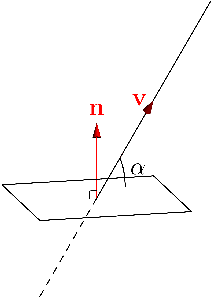
\includegraphics{figures/angle_between_line_and_plane.pdf}
        \end{center}
    \end{minipage}
    \begin{gather*}
        \sin\theta = \cos \angle (\vn, \vv) = \frac{Av_1 + Bv_2 + Cv_3}
        {\sqrt{A^2+B^2+C^2} \sqrt{v_1^2+v_2^2+v_3^2}}\\
        \alpha \parallel l_1: Av_1 + Bv_2 + Cv_3 = 0\\
        \alpha \perp l_1: \frac{A}{v_1} = \frac{B}{v_2} = \frac{C}{v_3}
    \end{gather*}
\end{definition}

\begin{theorem}
    TODO: Сделать рисунок

    $l_1, l_2$ -- пересекаются в одной точке или параллельны
    \[\Leftrightarrow
        \begin{vmatrix}
            x_1 - x_0 & y_1-y_0 & z_1-z_0 \\
            v_1       & v_2     & v_3     \\
            w_1       & w_2     & w_3
        \end{vmatrix} = 0\]
\end{theorem}
\begin{proof}
    $l_1$ и $l_2$ -- в одной плоскости, только если $\vv, \vw$ и
    $(x_1-x_0, y_1-y_0, z_1-z_0)$ в одной плоскости, это равносильно тому, что
    их смешанное произведение равно 0.
\end{proof}
\begin{example}
    $\perp$ к $l_1$ через $(x_1, y_1, z_1)$
    \begin{gather*}
        \frac{x-x_1}{A} = \frac{y-y_1}{B} = \frac{z-z_1}{C}\\
        \begin{cases}
            Av_1 + Bv_2 + Cv_3 = 0 \\
            \begin{vmatrix}
                x_1 - x_0 & y_1-y_0 & z_1-z_0 \\
                v_1       & v_2     & v_3     \\
                A         & B       & C
            \end{vmatrix} = 0
        \end{cases}
    \end{gather*}
\end{example}

\begin{definition}[Уравнение плоскости через прямую пересечения]
    TODO: Сделать рисунок
    \begin{gather*}
        \alpha_1: A_1x + B_1y +C_1z + D_1 = 0\\
        \alpha_2: A_2x + B_2y +C_2z + D_2 = 0
    \end{gather*}
    Уравнение пучка плоскостей, проходящих через прямую
    \begin{equation}\label{eq:two_lambdas}
        \lambda_1 (A_1x + B_1y +C_1z + D_1) + \lambda_2 (A_2x + B_2y +C_2z + D_2) = 0
    \end{equation}
    \begin{equation}\label{eq:one_lambda}
        \frac{\lambda_2}{\lambda_1} = \lambda \qquad
        A_1x + B_1y +C_1z + D_1 + \lambda (A_2x + B_2y +C_2z + D_2) = 0
    \end{equation}
    \[\lambda_1 = 0 \implies \lambda_2 \neq 0 \text{ считаем, что } \lambda_2 = 1
        \implies \text{уравнение } \alpha_2 \]
    \eqref{eq:one_lambda} описывает все плоскости проходящие, через прямую кроме $\alpha_2$.
\end{definition}


\begin{proposition}
    Любая плоскость через $l$ выражается через \eqref{eq:two_lambdas}.
\end{proposition}
\begin{proof}
    Если это $\alpha_2$ -- ок ($\lambda_1 = 0; \lambda_2 =1$).

    Если не $\alpha_2 \implies$ ищем \eqref{eq:one_lambda}:

    Искомая плоскость проходит через $(x_1, y_1, z_1)$:
    \begin{gather*}
        A_1 x_1 + B_1 y_1 + C_1 z_1 + D_1 + \lambda(A_2 x_1 + B_2 y_1 + C_2 z_1 + D_2) = 0\\
        \exists \lambda \text{ и находится через это уравнение }
    \end{gather*}
\end{proof}

Если три плоскости: $\alpha_1, \alpha_2, \alpha_3$,
хотим провести плоскость через общую точку пересечения

\begin{multline*}
    \lambda_1(A_1x + B_1y +C_1z + D_1) + \lambda_2 (A_2x + B_2y +C_2z + D_2)\\
    + \lambda_3 (A_3x + B_3y +C_3z + D_3)  = 0
\end{multline*}

\end{document}